\chapter{Introduction}
The continuing decline of print news readership
has been documented \cite{ma2014, nytimes2019}, alongside the
growth of online social networks (OSN), and their expanding role
in news dissemination \cite{goel2012}.  Within the space of
online news, there are highly automated news recommendation
services, or {\it news aggregators}.  Two popular news aggregators
are {\it Google News} and {\it Yahoo News}.  But there are many more niche news
aggregators.  In Sweden, a service named {\it Omni} exists,
focussing on multi-source news from a Swedish perspective.  In
information technology circles, {\it Hacker News} is popular, a news
aggregator by definition, with some social features.

There are open-source tools allowing people to create their own
aggregators, including {\tt tt-rss} \cite{ttrss} and Thunderbird's newsfeeds feature.
These open-source tools currently lack intelligent functionality
however, and sources must be added manually.  Some online news
sources aren't supported, if the website doesn't provide an RSS
or Atom feed link.

\subsection{The task\label{task}}
The task of personalised news aggregation is a complex one, but it can
be broken down into several more manageable tasks.  These tasks are
well described by the following questions:
\begin{enumerate}
    \item What is news?
    \item What is a news source?
    \item What is a good/bad news source?
    \item What is the official homepage of a news source?
    \item How do we discern article links on a homepage from other
          links (ads, etc.)?
    \item Who is the author of an article?
    \item When was an article released/published/printed?
    \item Which parts of a webpage actually correspond to article content,
          i.e. headline, byline, body, visual media and captions?
    \item What is a highly importance topic for the current
          news cycle?
    \item How do identify similar articles, and eliminate all but the best
          sources for that article?
    \item Is the {\it best source} the paper that ``got there first'', or
          the paper with highest rank, or the paper that covered the
          topic the best, or some other heuristic based on a
          combination of these metrics?
\end{enumerate}

\subsection{What is news?}
This question is mostly a philosophical one.  But for the practical
purposes of this project, an estimated answer is given by way of examples.
People may agree that things you read in a newspaper are news,
for example {\it The Irish Times}, {\it Reuters}, {\it The Financial
Times}.  But then there are other forms of media that lie in
an ontological sense somewhere between `online newspaper' and
`online radio station', or between `online newspaper' and
`quiz website' ({\it BuzzFeed}), or between `online newspaper' and
`TV station' ({\it BBC}).  For most of the examples given so far, at least
sometimes, these sources contain information people would describe as
news.  In this project, the answer to the question "Is something a
newssource?" is determined by supervised machine learning.  Different
encyclopedia pages are labelled with a binary class, {\it news source} or
{\it not news source}.  From this data, a program is generated that
takes unlabelled encyclopedia pages as input, and returns a probability
score that the encyclopedia page is a {\it news source}.

This pattern of supervised machine learning is repeated for several of the
questions surrounding news aggregation, including ``What is the
official homepage of a news source?'', ``Given a webpage that is an
article, what is the author of the article, the date the article was
published, and what is the headline?  The process is described in
more detail in Section \ref{ml}.

\section{Terminology}

Some news related and technical terminology are used throughout this
dissertation.  These terms will now be introduced.

\paragraph{Class} This term is used to mean some boolean or label
that can be applied to a document.  In most cases, boolean classes
({\it true} or {\it false}) are used instead of labels (many-valued
logic).  Though it is common to represent a document's class as a
real number between 0 and 1, 0 being {\it false} and 1 being
{\it true}.
\paragraph{False positive}
This defines a situation when a positive classification is made
incorrectly, e.g. when some fact is said to be true for a document,
when the fact does not actually hold true for that document.
\paragraph{False negative}
This defines a situation when a negative classification is made
incorrectly, e.g. when we {\it miss} a document for which a fact
would true.
\paragraph{True positive and true negative} As the names suggest, these
two terms indicate when a classification is made ({\it true} or
{\it false}), and the classification is correct.
\paragraph{News index}  This refers to certain kinds of webpages
that list a number of news items.  The category webpages within a
news website ({\it World}, {\it Sport}, etc.) are examples of
news indices.
\paragraph{News item}  This refers to webpages that contain news in
some longform way (a few paragraphs, a headline, etc.). 
The term {\it article} is avoided since it relates mostly to newspapers,
and \nr{} aims to process news from a broader category of online media.
\paragraph{Precision} This is the rate of accuracy within positive
classifications.  It can best be understood as a question: ``If
a classifier labels an item as positive, what is the likelihood
the correct label is in fact {\it positive}?''
\paragraph{Recall} The ratio of items correctly classified as positive
to the actual total of positives.  This measures how well a
classification system performs at the task of exhaustively finding
all positive items in a dataset.
\\\\
\noindent Accuracy is another popular term in machine learning (correct
classifications over total classifications), but that term is avoided
in this dissertation, because it can be misleading when classes are
not evenly distributed.  For example, a classifier that says
everything is a positive match would perform with 95\% accuracy
when 95\% of items just happen to be positive matches.

\section{The corpus}
\begin{wrapfigure}{r}{0.5\textwidth}
    \centering
    \fbox{
\includegraphics[width=0.3\textwidth]{media/official1.png}}
    \caption{
        The position of an `official homepage' link on a Wikipedia
        webpage's {\tt vcard} (highlighted in yellow).
        \label{official1}
    }
\end{wrapfigure}
As will be discussed in Section \ref{corpus}, the unstructured web
poses a challenge to structured data extraction. In Figures
\ref{official1} and \ref{official2}, three different
positions for `official homepage' links appear on
newspapers' Wikipedia articles.  An intelligent web scraper is
needed, capable of recognising all different scenarios, and extracting
the links most likely to represent official homepages.

Another task arises after the official homepages for news sources
are determined.  Which links on a homepage or other
index page correspond to news items and other news indices?
(Figures \ref{index1} and \ref{index2})

\begin{figure}[H]
    \centering
    \fbox{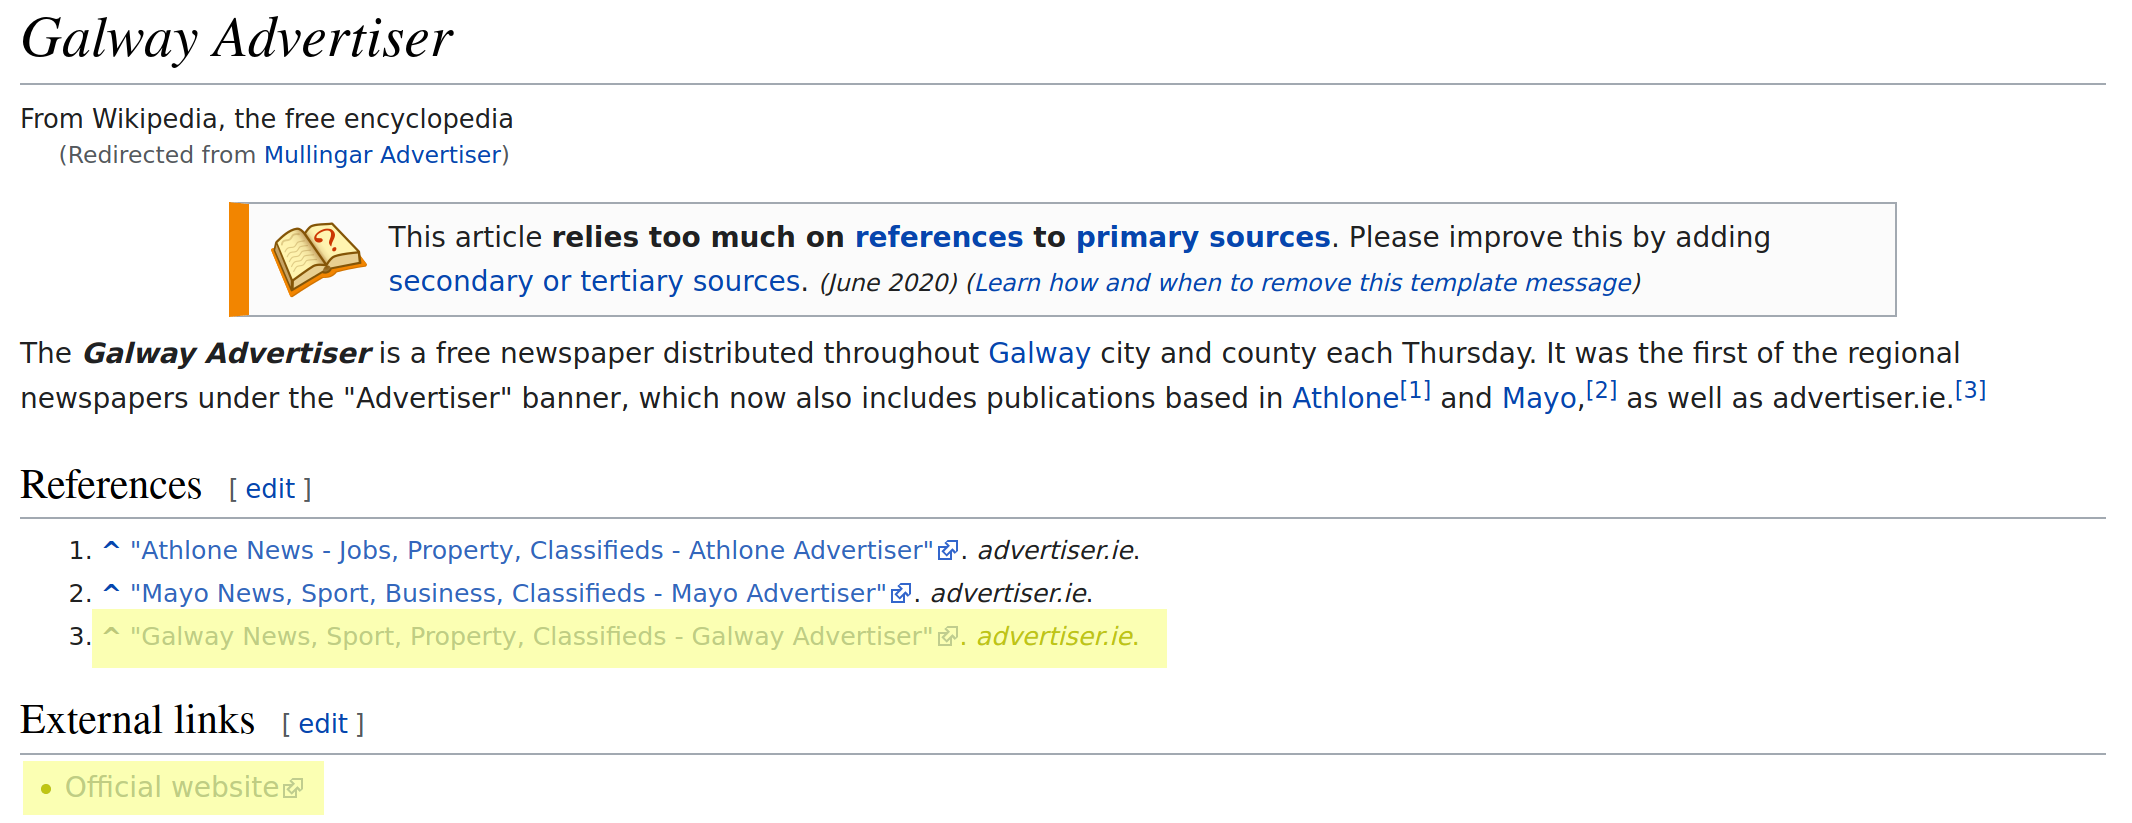
\includegraphics[width=0.8\textwidth]{media/official2.png}}
    \caption{
        \raggedright
        The position of official homepage links at the bottom
        of another Wikipedia webpage.\label{official2}
    }
\end{figure}
\begin{figure}[H]
    \centering
    \fbox{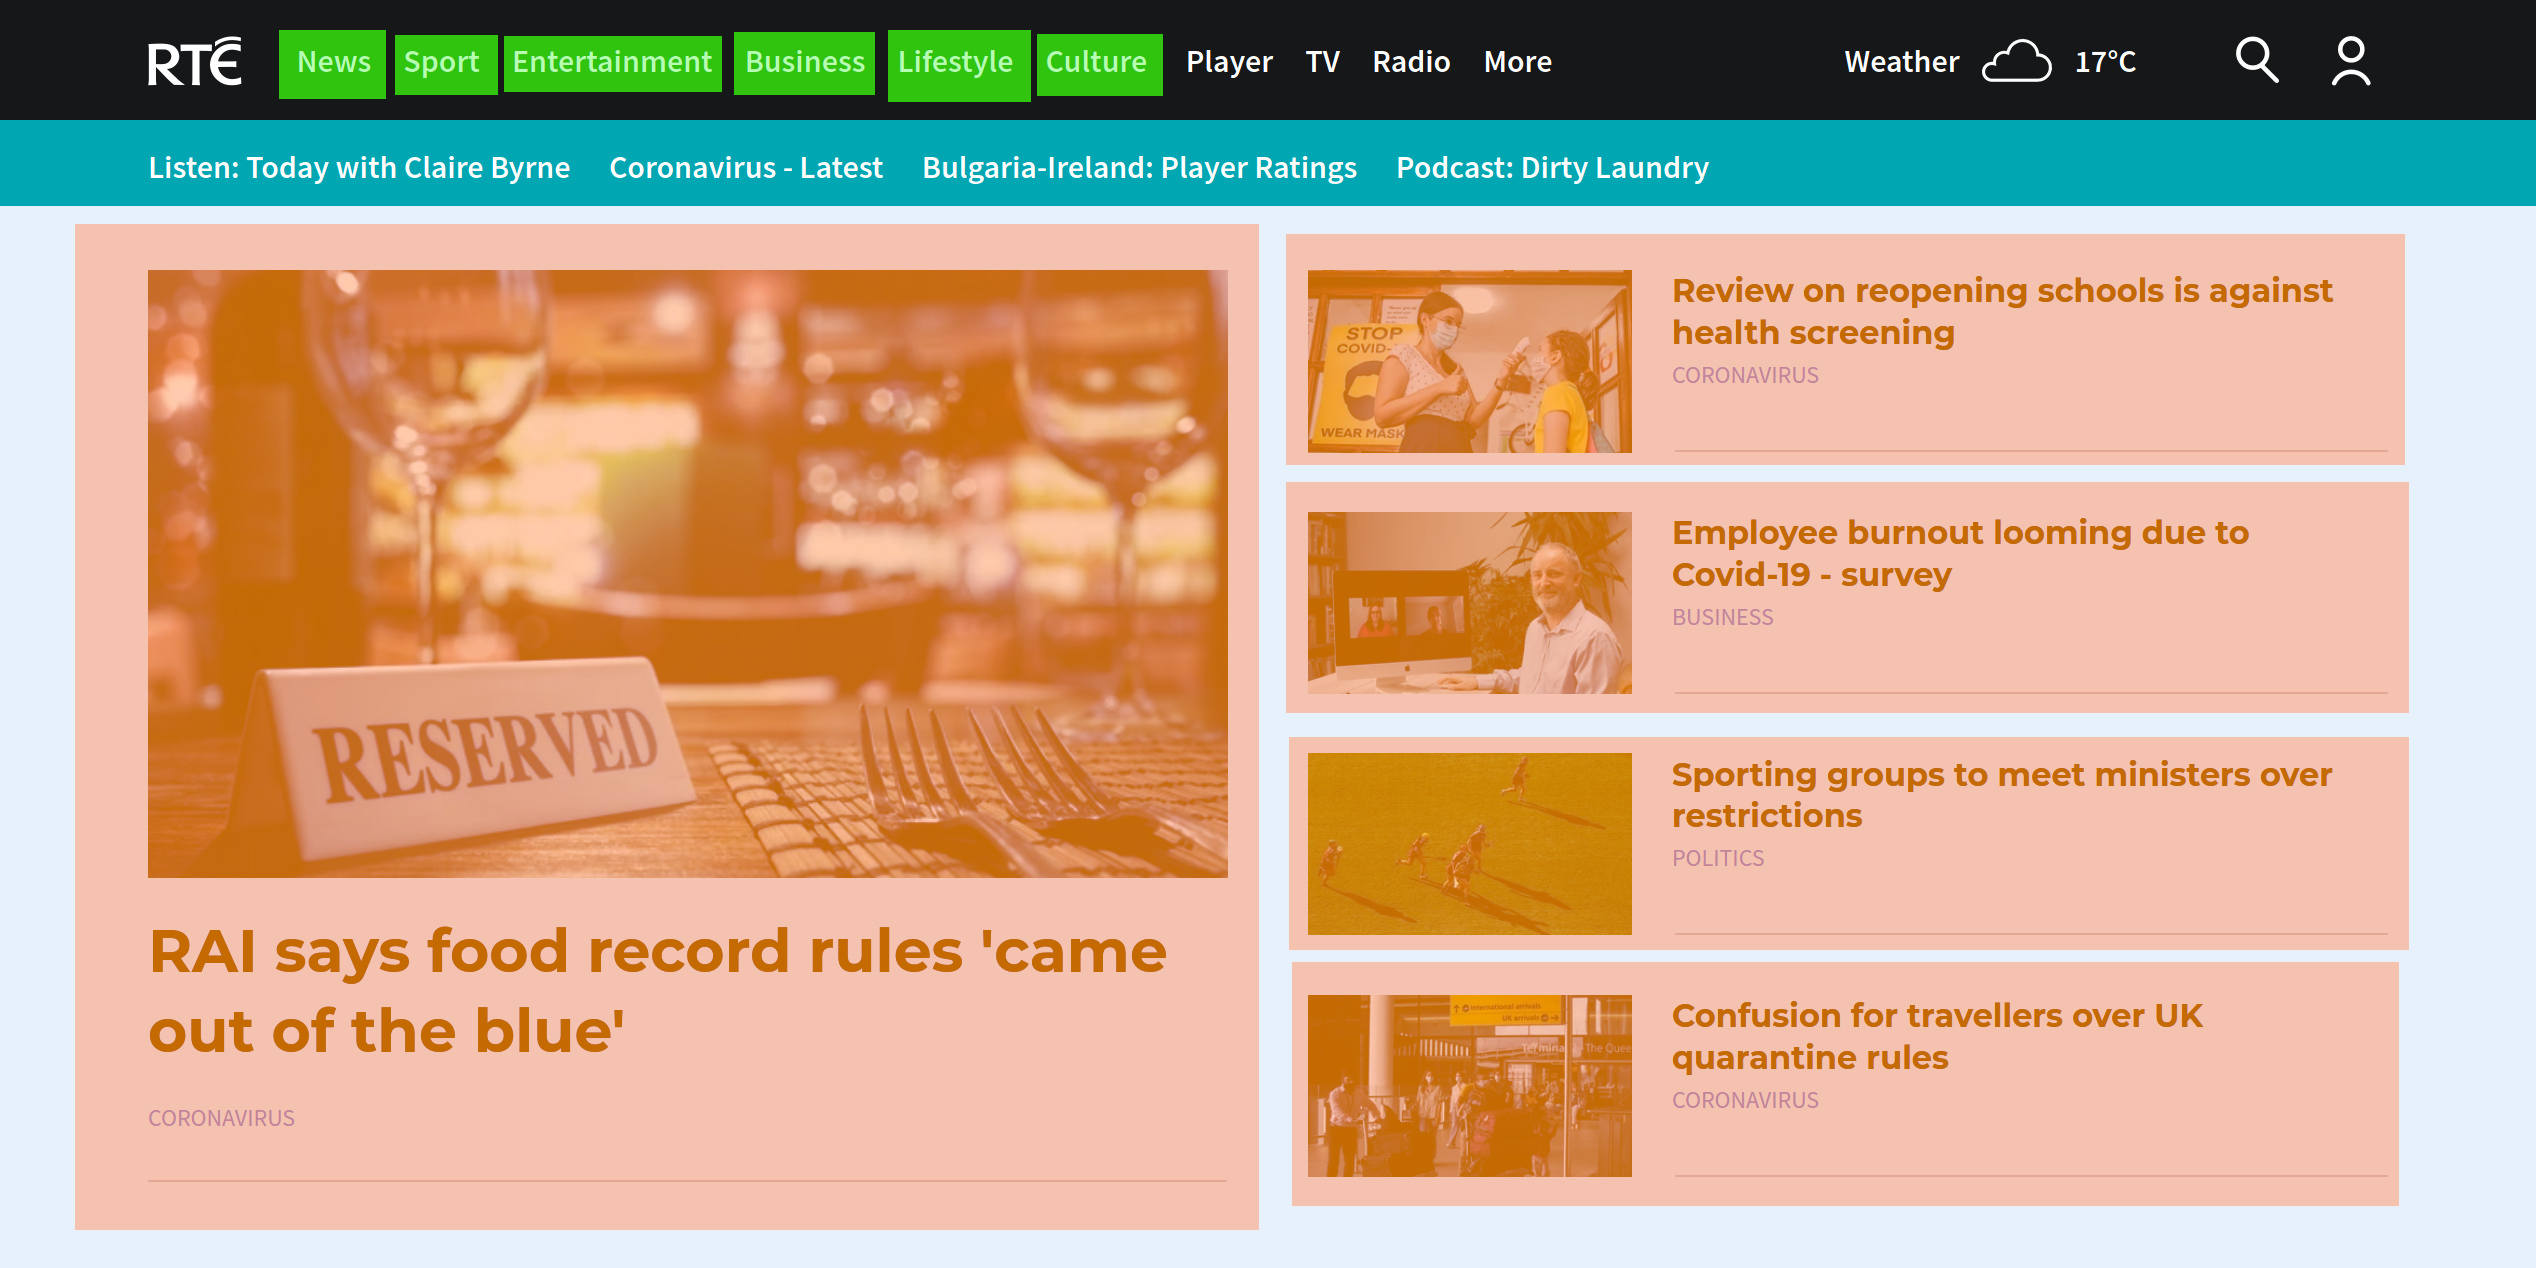
\includegraphics[width=0.8\textwidth]{media/index.png}}
    \caption{
        Index links (green) and item links (orange)
        on the RTE homepage.\label{index1}
    }
\end{figure}
\begin{figure}[H]
    \centering
    \fbox{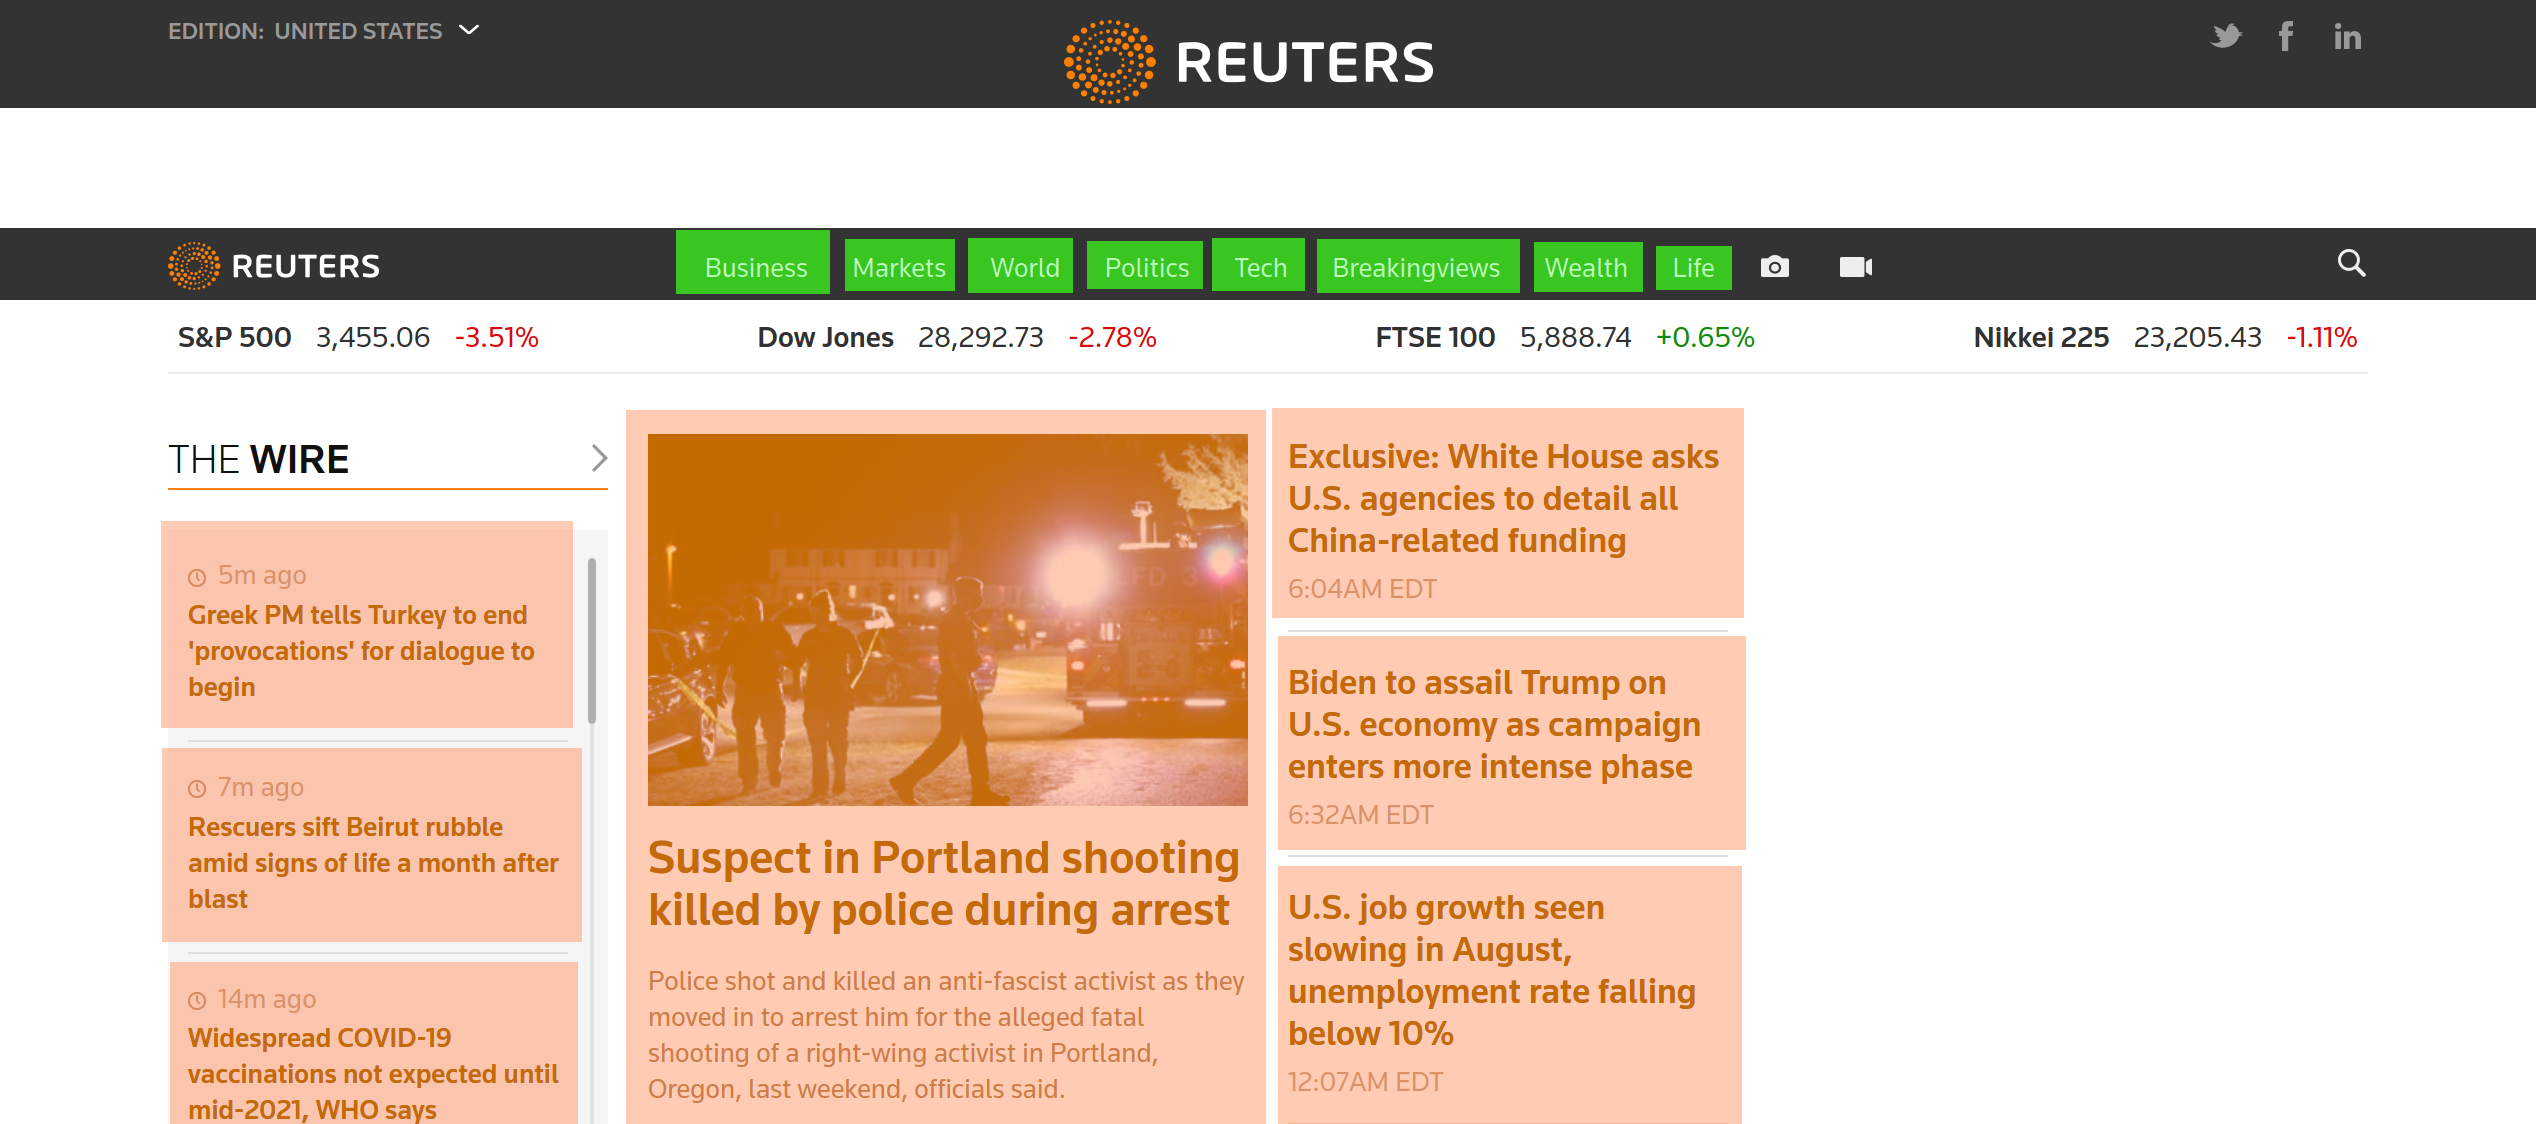
\includegraphics[width=0.8\textwidth]{media/index2.png}}
    \caption{
        Index links (green) and item links (orange)
        on the Reuters homepage.\label{index2}
    }
\end{figure}\clearpage

Within news items on each page, there are several more relation
extraction tasks.  Figures \ref{item1} and \ref{item2} show some of
the key labelled information associated with news items.  Note that
in one news item (\ref{item1}), there is a single author, and in the
other there are two authors (\ref{item2}).  The publication date is
labelled relatively in one news item, ``a day ago'', and literally
in the other news item.  One news item has a byline, the other one
doesn't.
\begin{figure}[H]
    \centering
    \fbox{
\includegraphics[width=0.7\textwidth]{media/item1.png}}
    \caption{Information of interest on a news item page:
    publication date (pink), headline (blue), byline (red),
    author name (purple).\label{item1}
    }
\end{figure}
\begin{figure}[H]
    \centering
    \fbox{
\includegraphics[width=0.7\textwidth]{media/item2.png}}
    \caption{The same information types from Figure \ref{item1},
    on a different news item page.\label{item2}}
\end{figure}
\noindent The underlying {\tt HTML} for each of these webpages
also varies greatly.  This level of variance necessitates
a dynamic, probabalistic approach to web scraping, rather than
manually writing rules based on the assumption of semantically
correct and uniform {\tt HTML}.

With a firm grasp on the tasks, terminology, and the structure the
dataset will take, the next chapter will cover background research
related to these tasks.